% -----------------------------------------------
% Vlastní text práce (kapitoly práce)
% -----------------------------------------------

% -----------------------------------------------
\chapter{Instrumentation}
% -----------------------------------------------
To perform all of necessary measurements we need to use various types of optical and electronic equipment, which is discussed in this chapter.
% -----------------------------------------------
\section{Integration sphere}
% -----------------------------------------------
The Integration sphere (IS) is a special optical equipment, which can be used either as extended uniform light source (EULS) e.g. with spectrometer in determining the material reflectance. In our experiments we use general purpose Labsphere (Fig. \ref{Labsphere}).

\begin{figure}[H]
 \centering
 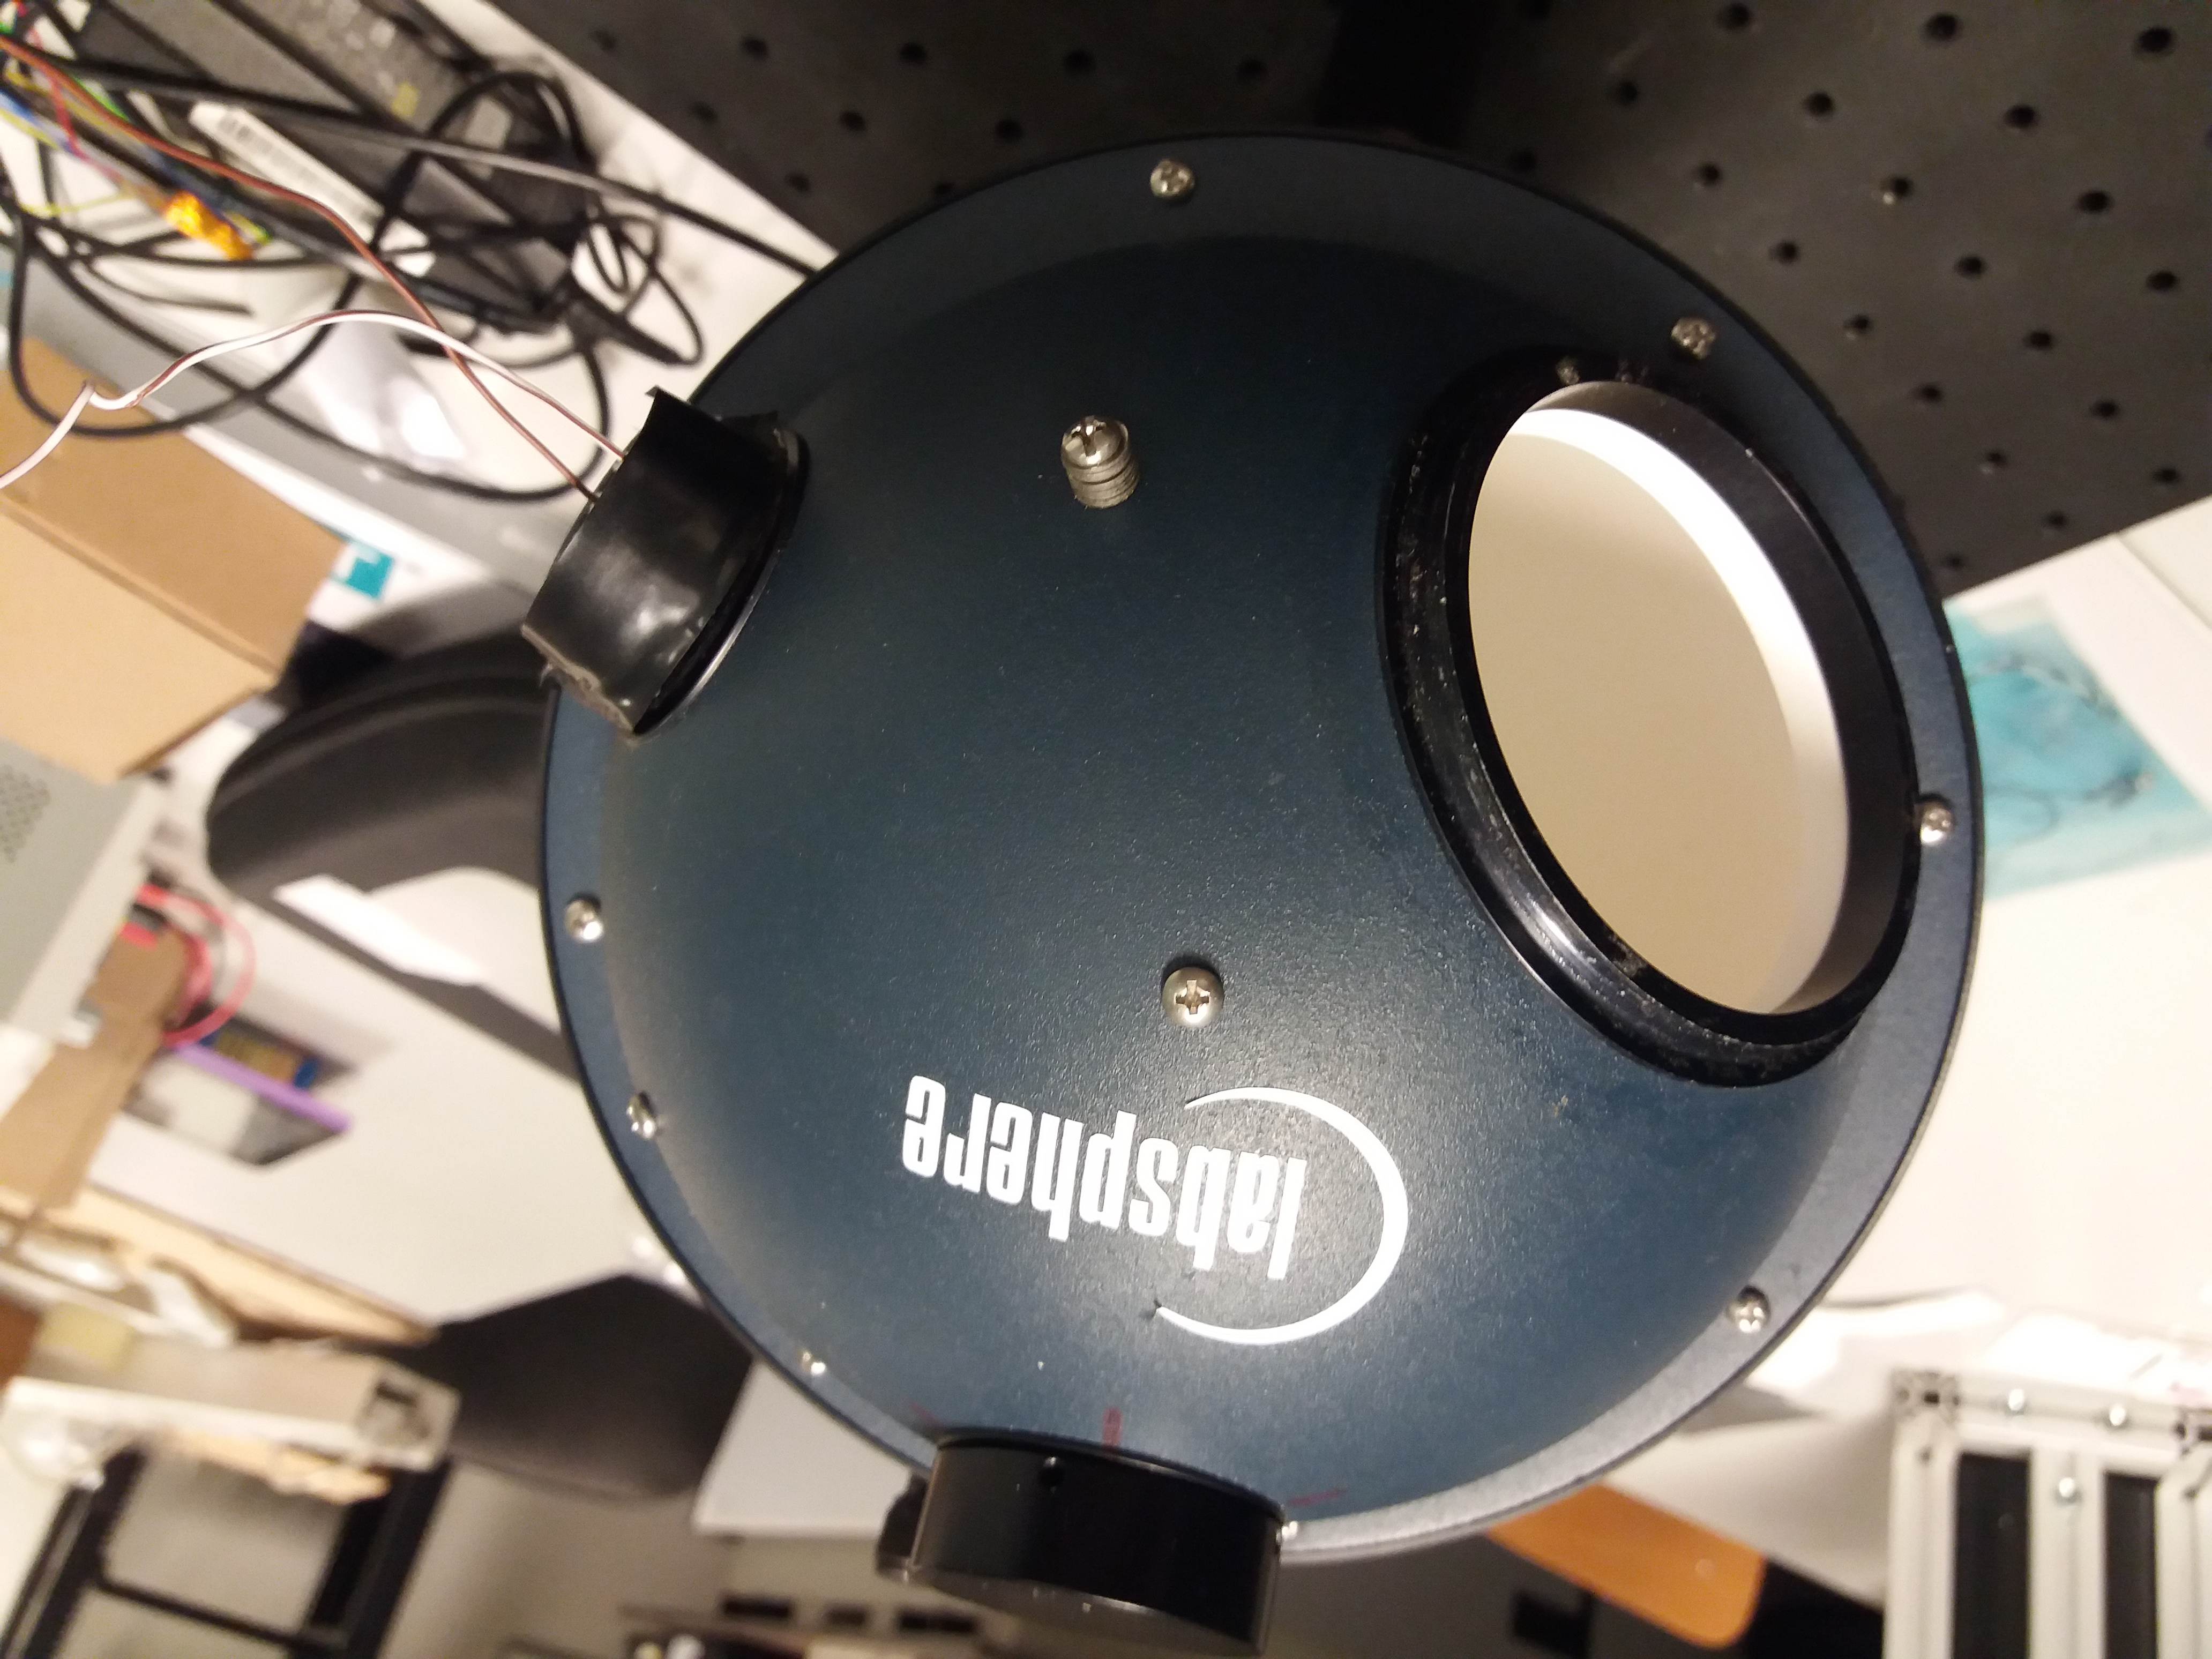
\includegraphics[scale=0.09, angle = 180]{./pictures/IntegrationSphere}
 \caption{General purpose Labsphere.}
 \label{Labsphere}
 
\end{figure}
\par
The IS inner surface consist of white optical diffusive material (BaSO$_4$ and Polytetrafluoroethylene). The IS also contains several circular apertures, which are called input/output ports. These can be used to mount detectors or optical sources or left free to let light flux enter or exit IS. 
\par
The inner surface is the part where light integration happens. The effect which takes place here is known as Lambertian scattering. After one spot of inner surface is hit by a ray, the energy should be uniformly radially distributed. In output port this produces a homogeneous light source. The homogeneity decreases with increasing number and sizes of input/output ports.
\par
Using optical source with IS typically requires baffle to prevent source's light flux or its part to exit IS without integration.
\par
Deep explanation of IS working principles and characterization of optical properties of the identical IS, which we use, can be found in \cite{VACULA2021167169}.
\par
For our purposes, in case of FAST calibration, we use IS as an UV EULS. In case of testing optical UV calibration source, we use IS mainly to block the possible incoming external light and to distribute the optical power of the UV source between mounted detectors.
% -----------------------------------------------

\section{Photomultiplier tube}
% -----------------------------------------------
Photomultiplier tube (PMT) is considered to be a high voltage optoelectronical part. It allows us to measure very low intesity optical signals. PMT is also characterized by high amplification, low noise and stability. It has many variants of usage. It can be used either as detector of optical signal (pulse or continual) for chosen wavelength or as a radiation detector. The general theory of PMTs is described in more detail in \cite{Photonis, Hamamatsu}. 
\subsection{Operating principle}
PMT consists of 6 main elements, which can be seen on scheme \ref{PMT scheme}.

\begin{figure}[H]
 \centering
 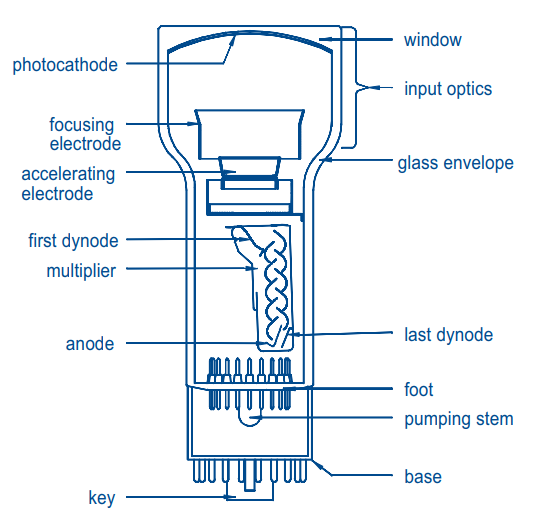
\includegraphics[scale = 0.5]{./pictures/PMTscheme}
 \caption{Photomultiplier tube scheme \cite{Photonis}.}
 \label{PMT scheme}
\end{figure}

\begin{figure}[H]
 \centering
 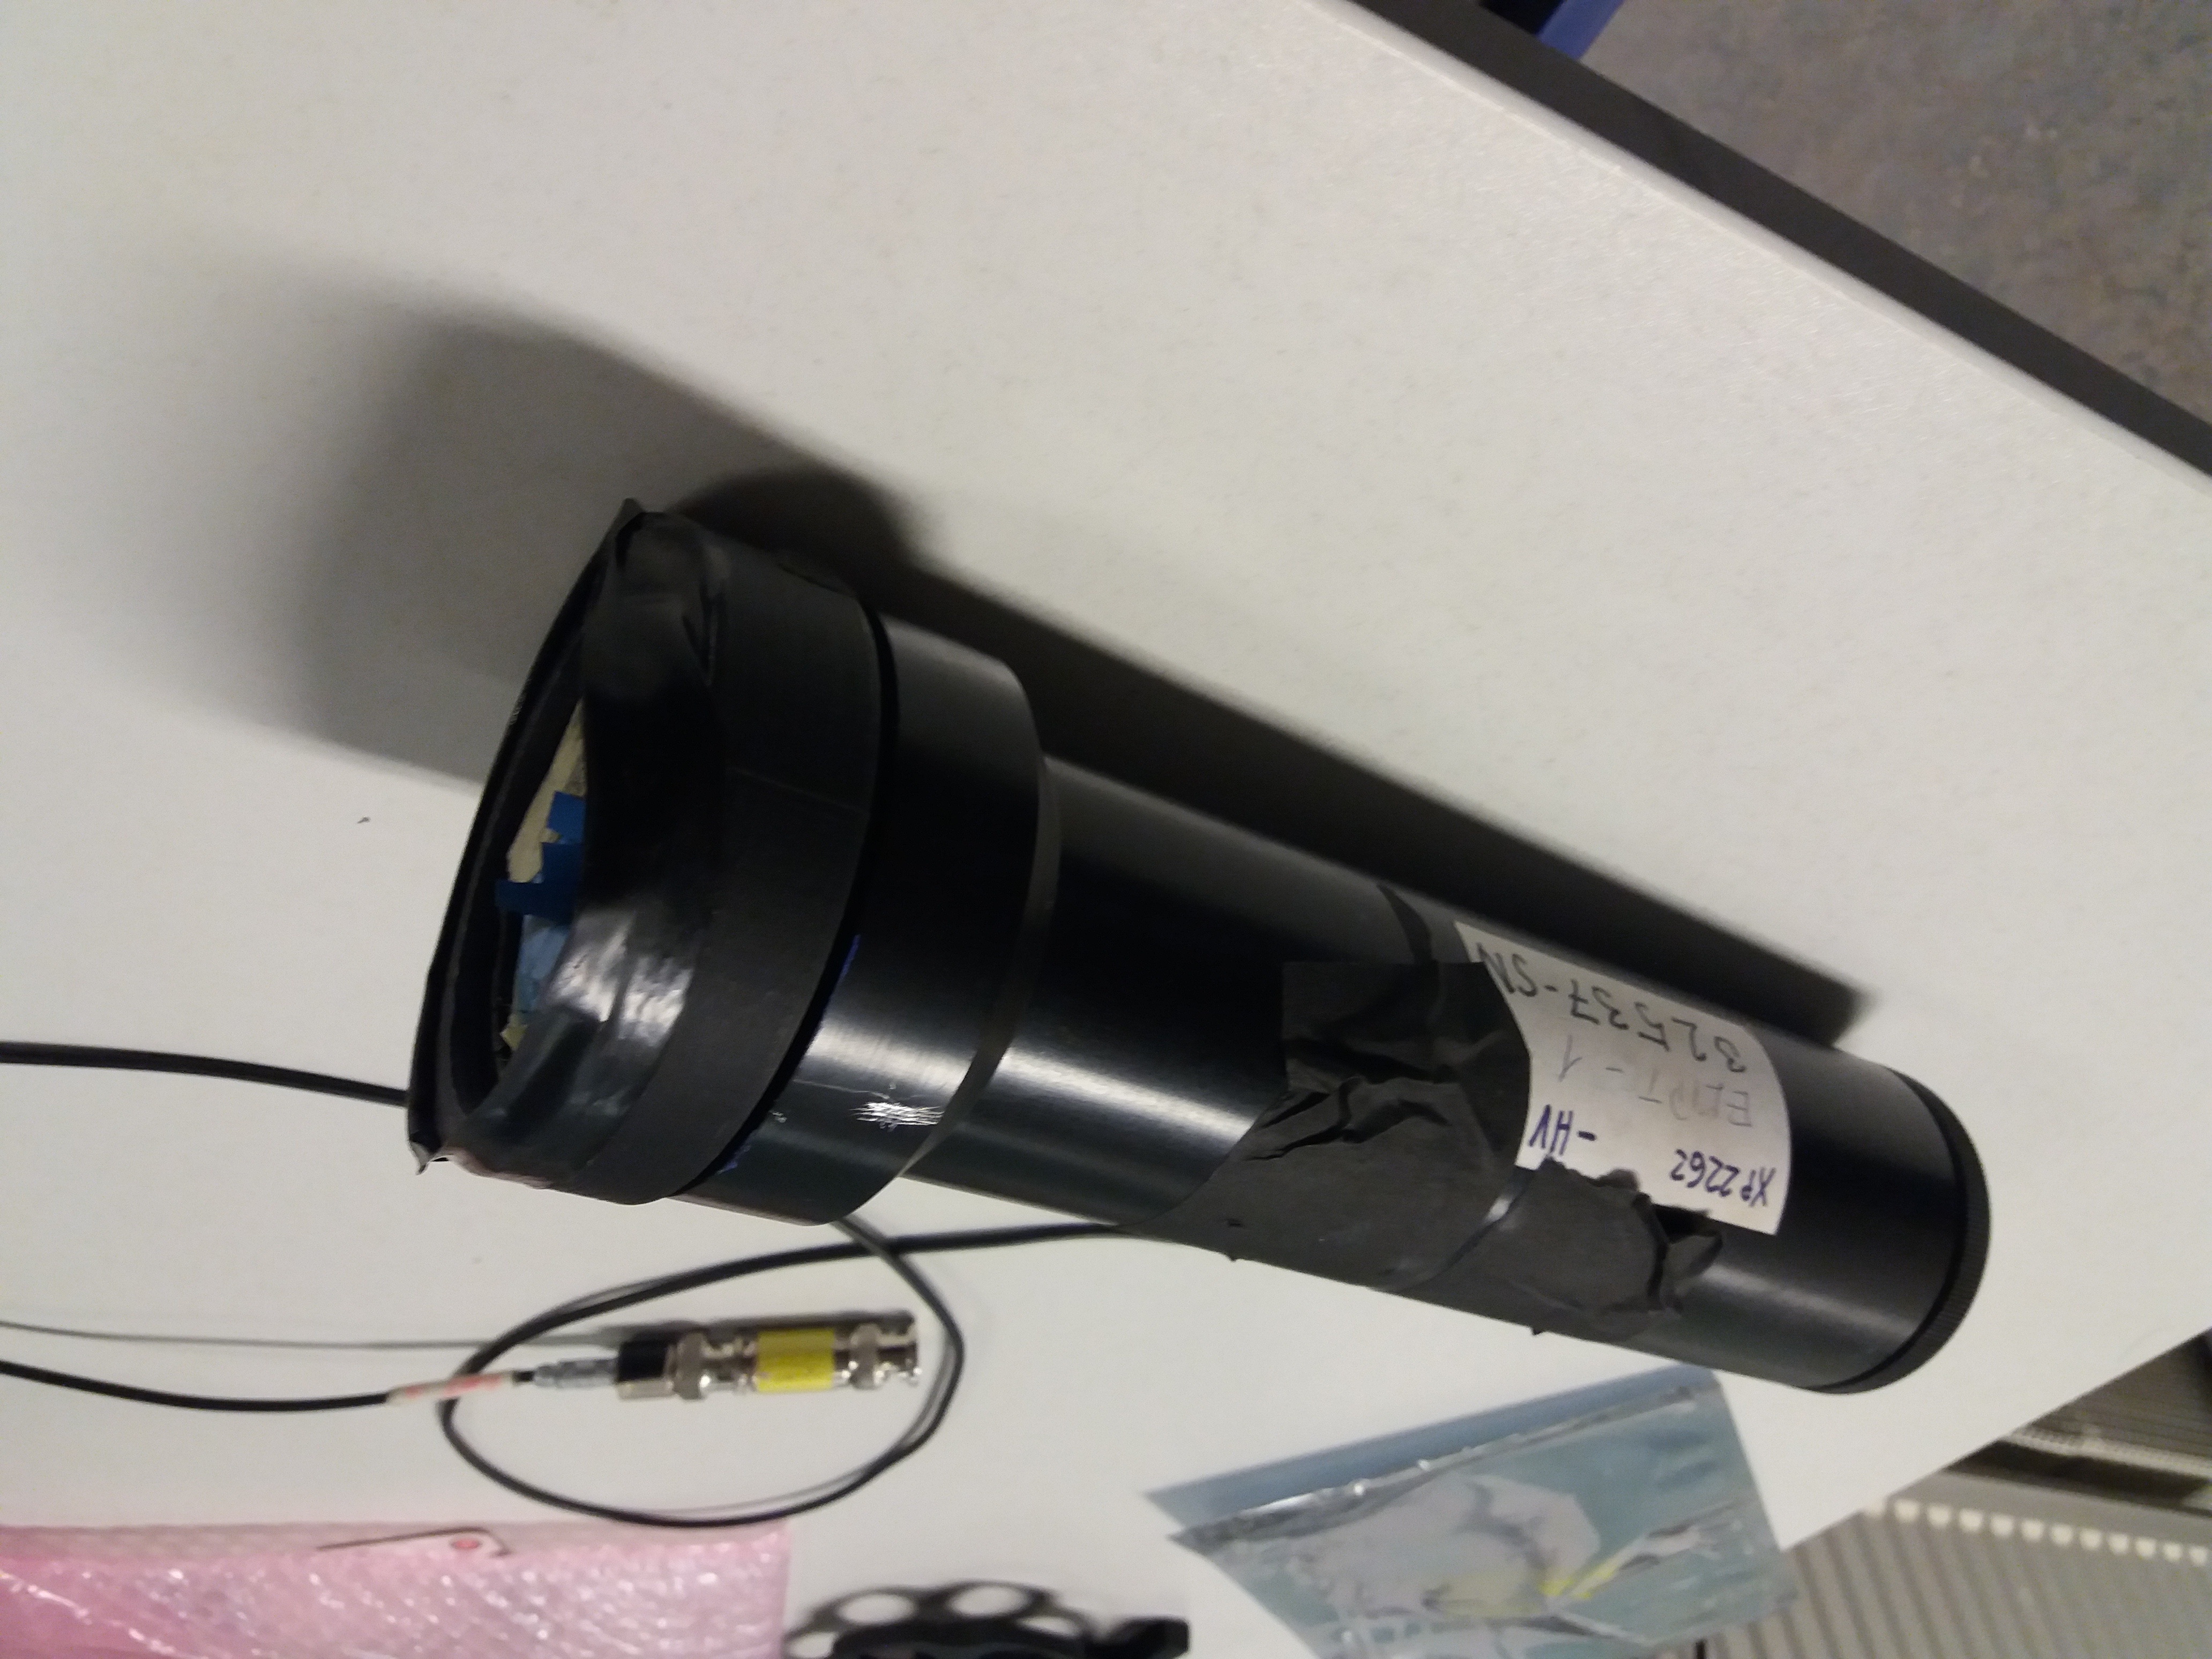
\includegraphics[scale = 0.08, angle = 180]{./pictures/XP2262}
 \caption{XP2262 PMT in a metal enclosure used for our measurements.}
 \label{XP2262 PMT}
\end{figure}

\par
The input photon with sufficient energy, which strikes the PMT's photocathode, excites photocathode's electron. This electron then follows electrostatic field to the first dynode of the electron multiplier, where it induces secondary emission of more electrons. These electrons are then attracted by the next dynode, where the emission process repeats. After few times of multiplying electron number over dynodes, the electrons are then collected by 
the anode, which is situated on the end of the electron multiplier. The anode output current is then converted to voltage signal by appropriate load resistor or by operational amplifier current-to-voltage circuit.
\par
As all other laboratory instruments, which are based on accelerating electrons, such as electron microscopes, the photomultiplier's main parts must be kept in vacuum. To maintain vacuum, the photomultiplier is surrounded by special glass envelope. To avoid mechanical damage of the glass envelope, the entire photomultiplier is sometimes situated in a plastic tube.
\par
One of the basic adjustable characteristics of PMT is its gain. The gain is defined as:

\begin{equation}
G = \frac{I_\textrm{a}}{I_\textrm{p}},
\end{equation}
where $I_\textrm{a}$ is the anode current and $I_\textrm{p}$ is the input photocurrent from the photocathode.
\par
In case of ideal, noiseless PMT, we can adjust gain by varying the supply voltage. By varying supply voltage we can adjust gain according to an equation:

\begin{equation}
\frac{G_2}{G_1} = (\frac{V_2}{V_1})^{\alpha N},
\label{gainVolt}
\end{equation}
where $G_2$ and $G_1$ are gains at supply voltages $V_2$ and $V_1$. $\alpha$ is coefficient given by dynode material and $N$ is the number of dynodes.
\par
Other effects, such as temperature, may also vary PMT's gain, and it is necessary to keep them on constant value or measure them and involve them in the final evaluation of data.
\par
For the proper functionality of the PMT, the charge and current linearity should be considered. Charge linearity is the ratio of the number of incident photons to the number of electrons collected at the anode. Current linearity expresses the proportionality between incident light flux and anode current. Ideal PMT is always linear, but the real PMT may vary from linearity due to drifts, space charges, instability of voltage divider etc. These effects can lead up to saturation of the PMT. In saturation, increasing the input light flux leaves the anode current mostly unchanged.      


\subsubsection{Window}

The photocathode is coated on glass window, whose main purpose is to admit light of certain wavelengths. Glass materials are characterized by the spectral sensitivity to wavelengths. For transparency in UV spectre, it is advised to use borosilicate or fused silica glasses.


\subsubsection{Photocathode}

The photocathode is the only light-sensitive part of PMT. It transfers the light flux into the electric current.
\par
One of its main parameters is quantum efficiency. It is referred to as ratio of emitted photoelectrons to the number of incident photons expressed as a percentage. It is generally less than 35 \%. For measurement, the more practical parameter is cathode radiant sensitivity. It is the ratio of photocathode current to an incident light power, which is expressed in mA/W.
\par
Photocathode material must be sensitive to certain wavelengths, which we want to detect with the PMT, and must have sufficient quantum efficiency. Preferred materials are usually alkali antinodes.
\subsubsection{Electron multiplier}
The electron multiplier consists of dynodes and one anode.
Dynodes are electrodes, which produce more electrons through secondary emission. To maintain electrostatic field between dynodes, each of dynodes is held on different potential. This is achieved by using the voltage divider. Every resistor in the divider sets the potential of one diode according to its resistivity.
\par
All of the photoelectrons emitted by photocathode should be ideally collected by the first dynode. However, many of them could be diverted from their path to dynode due to various effects. The parameter, which characterizes this, is the collection efficiency. The collection efficiency is probability that a photoelectron will strike area of the first dynode. 
\par
There are few types of dynodes arrangements. On the fig. \ref{PMT scheme} is the classic linear-focusing multiplier. 


\subsubsection{Voltage divider and voltage adjustment}
Voltage divider could be a simple resistor serial network, which divide high input voltage between the dynodes. 
\par
It is necessary to consider, that the multiplier current density increases in direction to the anode, so it tends to lessen the voltage between last dynode and anode. This phenomena can shake the potential levels across the entire multiplier. One way to reduce the impact on PMT's behaviour is to choose the proper resistor values of the divider. 
\par
The resistor values could same for all the dynodes, but for some applications it is better to have progressive voltage distribution, which increases from cathode to anode, or intermediate distribution with highest values on the beginning of the multiplier.

\par
In some applications, where high anode current peaks are expected, the divider can be filled with reservoir capacitors, which prevent the temporally charge exhaustion of the dynodes. In pulse mode, the unwanted oscillations on dynodes may occur, in that case, it is desirable to connect additional damping resistor to the divider.
\par
Voltage supply should be stable during the PMT's operation. As was mentioned before, the PMT's gain is voltage dependent. To adjust sufficient gain, high voltage (hundreds of volts) needs to be applied between photocathode and anode. The high voltage needs to be ramped on required level gradually to avoid negative consequences of transition and dark current effects, which can decrease the operating life of PMT. The same is valid for shutting down the PMT.
\par
The high voltage could be applied to the PMT in negative or positive polarity. In case of positive polarity, the cathode is held at ground and anode on +HV. In case of negative polarity, the cathode is held at -HV and anode at ground. 

\subsection{Dark current}
Dark current is the anode current produced by a photomultiplier in total darkness. It is considered to be a part of unwanted noise, causes errors in measurements and limits the detectivity of PMT. Dark current has origin in ohmical leakage, thermionic and field emission or in radioactivity. Ohmical leakage is major part of dark current at low gain. With the increasing gain the thermionic emission prevails. At high gains the field emission becomes the major part.
%\subsubsection{Ohmical leakage}
%Insufficent insulation of electrodes, dynodes and all other parts which are under high voltage may lead to surface current over glass and tube. Dirt and humidity are in most cases the reason of Ohmical leakage.

%\subsubsection{Thermionic emission}
%Temperature causes emission of photocathode's electrons, which are at medium gains the major part of dark current.  Due to this effect, some PMTs may need to be cooled during operation.
%\subsubsection{Field emission}
%At high gains the electrostatic field is so strong that it can rip the electrons out of the electrodes and accelerate them onto other surfaces, where they cause secondary emission. Field emission rapidly increases with supply voltage. In some literature it is also refered as cold emission.
%\subsubsection{Radioactivity}
%The radioactivity of PMT's components depends only on the material composition. In some aplications, such as astroparticle detection, it is neccessary to decrease radiation as possible. In astroparticle detection the radioactivity could be a source of false events. Only way to prevent this is to use materials with a very low concentration of radioactive isotopes.

\subsection{Timing and response}
Differences of photoelectrons' trajectories from the cathode to the first dynode lead into time distortion of signal. For example if we were able to produce delta-function pulse, the PMT would detect pulse with some response width time $t_\textrm{w}$.
With respect to differences in electron trajectories and arrival times, the PMTs are divided into 3 types:
\begin{enumerate}
\item \textbf{Very-fast tubes} - photoelectrons arrive simultaneously, low collection efficiency.
\item \textbf{Fast tubes} - compromise between timing performance and collection efficiency
\item \textbf{General-purpose tubes} - simple optoelectronics, good collection efficiency, low timing performance
\end{enumerate}
%\par 
%Another time delay to be considered 

\subsection{Operating life and degradation}
The operating life of PMT is defined as the time required for anode sensitivity to be halved. If we neglect the outside effects, the operating life mainly depends on anode current. 
Degradation processes start to show themselves at currents higher than 10 $\mu$A. Ageing is accompanied by increasing or decreasing gain at stable voltage. Operating life of PMT is measured in thousands of operating hours.
\par
By exposing PMT to bad conditions, such as humidity, mechanical stress, high temperatures or the high-intensity light, the PMT's operating life could be shorten much faster.
%------------------------------------------------
%------------------------------------------------

\section{Hardware for experiment control}
% -----------------------------------------------

\subsection{Raspberry Pi}
Raspberry Pi (RPi) is a single board computer which we use mainly for the experiment control. The linux-based Raspbian or DietPi operating system allows us to easily run various scripts and programs written in multiple languages. By having wifi and an ethernet port, the RPi can be easily accessed over internet. It can be used to control instruments and data acquisition over its USBs,1-Wire and I2C etc. However, it doesn't have any analog inputs/outputs such as ADCs and DACs.
\subsection{STM32 based microcontrolers}
For other types of tasks, which do not require data storage and remote control, but require for example an analog sampling, setting up the voltage levels or generating well defined PWM pulses, we use STM32 based microcontrollers. 
\par
For this thesis purposes we use the STM32 nucleo F411RE and the STM32 nucleo F446RE with better analog inputs/outputs.
% -----------------------------------------------
% %%%%%%%%%%%%%%%%%%%%%%%% End of file %%%%%%%%%%%%%%%%%%%%%%%%
